% Created 2018-04-30 Mon 11:12
\documentclass[11pt]{article}
\usepackage[utf8]{inputenc}
\usepackage[T1]{fontenc}
\usepackage{fixltx2e}
\usepackage{graphicx}
\usepackage{longtable}
\usepackage{float}
\usepackage{wrapfig}
\usepackage{rotating}
\usepackage[normalem]{ulem}
\usepackage{amsmath}
\usepackage{textcomp}
\usepackage{marvosym}
\usepackage{wasysym}
\usepackage{amssymb}
\usepackage{hyperref}
\tolerance=1000
\author{LAPTOP-33DVDSGR}
\date{\today}
\title{workflow}
\hypersetup{
  pdfkeywords={},
  pdfsubject={},
  pdfcreator={Emacs 24.5.1 (Org mode 8.2.10)}}
\begin{document}

\maketitle
\tableofcontents

\section{1)Concatenate the lanes for R1 and R2  for each replicate}
\label{sec-1}
\subsection{a)czar$_{\text{concat}}$.sh}
\label{sec-1-1}
\subsection{b)santana$_{\text{concat}}$.sh}
\label{sec-1-2}
\subsection{c)xerdo$_{\text{concat}}$.sh}
\label{sec-1-3}
\subsection{d)brach$_{\text{concat}}$.sh}
\label{sec-1-4}
\subsection{e)xellus$_{\text{concat}}$.sh}
\label{sec-1-5}
\subsection{f)zeus$_{\text{concat}}$.sh}
\label{sec-1-6}
\subsection{g)bigsby$_{\text{concat}}$.sh}
\label{sec-1-7}
\subsection{h)xadius$_{\text{concat}}$.sh}
\label{sec-1-8}
\section{2)Run HISAT2 [[/scratch/user/jochum/}
\label{sec-2}
\subsection{a)czar$_{\text{concat}}$.sh}
\label{sec-2-1}
\subsection{b)santana$_{\text{HIST}}$.sh}
\label{sec-2-2}
\subsection{c)xerdo$_{\text{HISAT}}$.sh}
\label{sec-2-3}
\subsection{d)brach$_{\text{HISAT}}$.sh}
\label{sec-2-4}
\subsection{e)xellus$_{\text{HISAT}}$.sh}
\label{sec-2-5}
\subsection{f)zeus$_{\text{concat}}$.sh}
\label{sec-2-6}
\subsection{g)bigsby$_{\text{concat}}$.sh}
\label{sec-2-7}
\subsection{h)xadius$_{\text{concat}}$.sh}
\label{sec-2-8}
\section{3)Run Stringtie}
\label{sec-3}
\subsection{a)czar$_{\text{stringtie}}$}
\label{sec-3-1}
\subsection{b)santana$_{\text{stringtie}}$.sh}
\label{sec-3-2}
\subsection{c)xerdo$_{\text{stringtie}}$.sh}
\label{sec-3-3}
\subsection{d)brach$_{\text{stringtie}}$.sh}
\label{sec-3-4}
\subsection{e)xellus$_{\text{stringtie}}$.sh}
\label{sec-3-5}
\subsection{f)zeus$_{\text{stringtie}}$.sh}
\label{sec-3-6}
\subsection{g)bigsby$_{\text{stringtie}}$.sh}
\label{sec-3-7}
\subsection{h)xadius$_{\text{stringtie}}$.sh}
\label{sec-3-8}
\section{4)Run Stringtie Merge}
\label{sec-4}
\subsection{a)fast}
\label{sec-4-1}
\subsection{b)slow}
\label{sec-4-2}
\subsection{c)unaffected}
\label{sec-4-3}
\section{5)Run Maker}
\label{sec-5}
\subsection{a)fast}
\label{sec-5-1}
\subsection{b)slow}
\label{sec-5-2}
\subsection{c)unaffected}
\label{sec-5-3}
\section{6)gffcompare}
\label{sec-6}
\subsection{a)maker files}
\label{sec-6-1}
\subsection{b)stringtie files}
\label{sec-6-2}
\section{Results}
\label{sec-7}
\begin{figure}[htb]
\centering
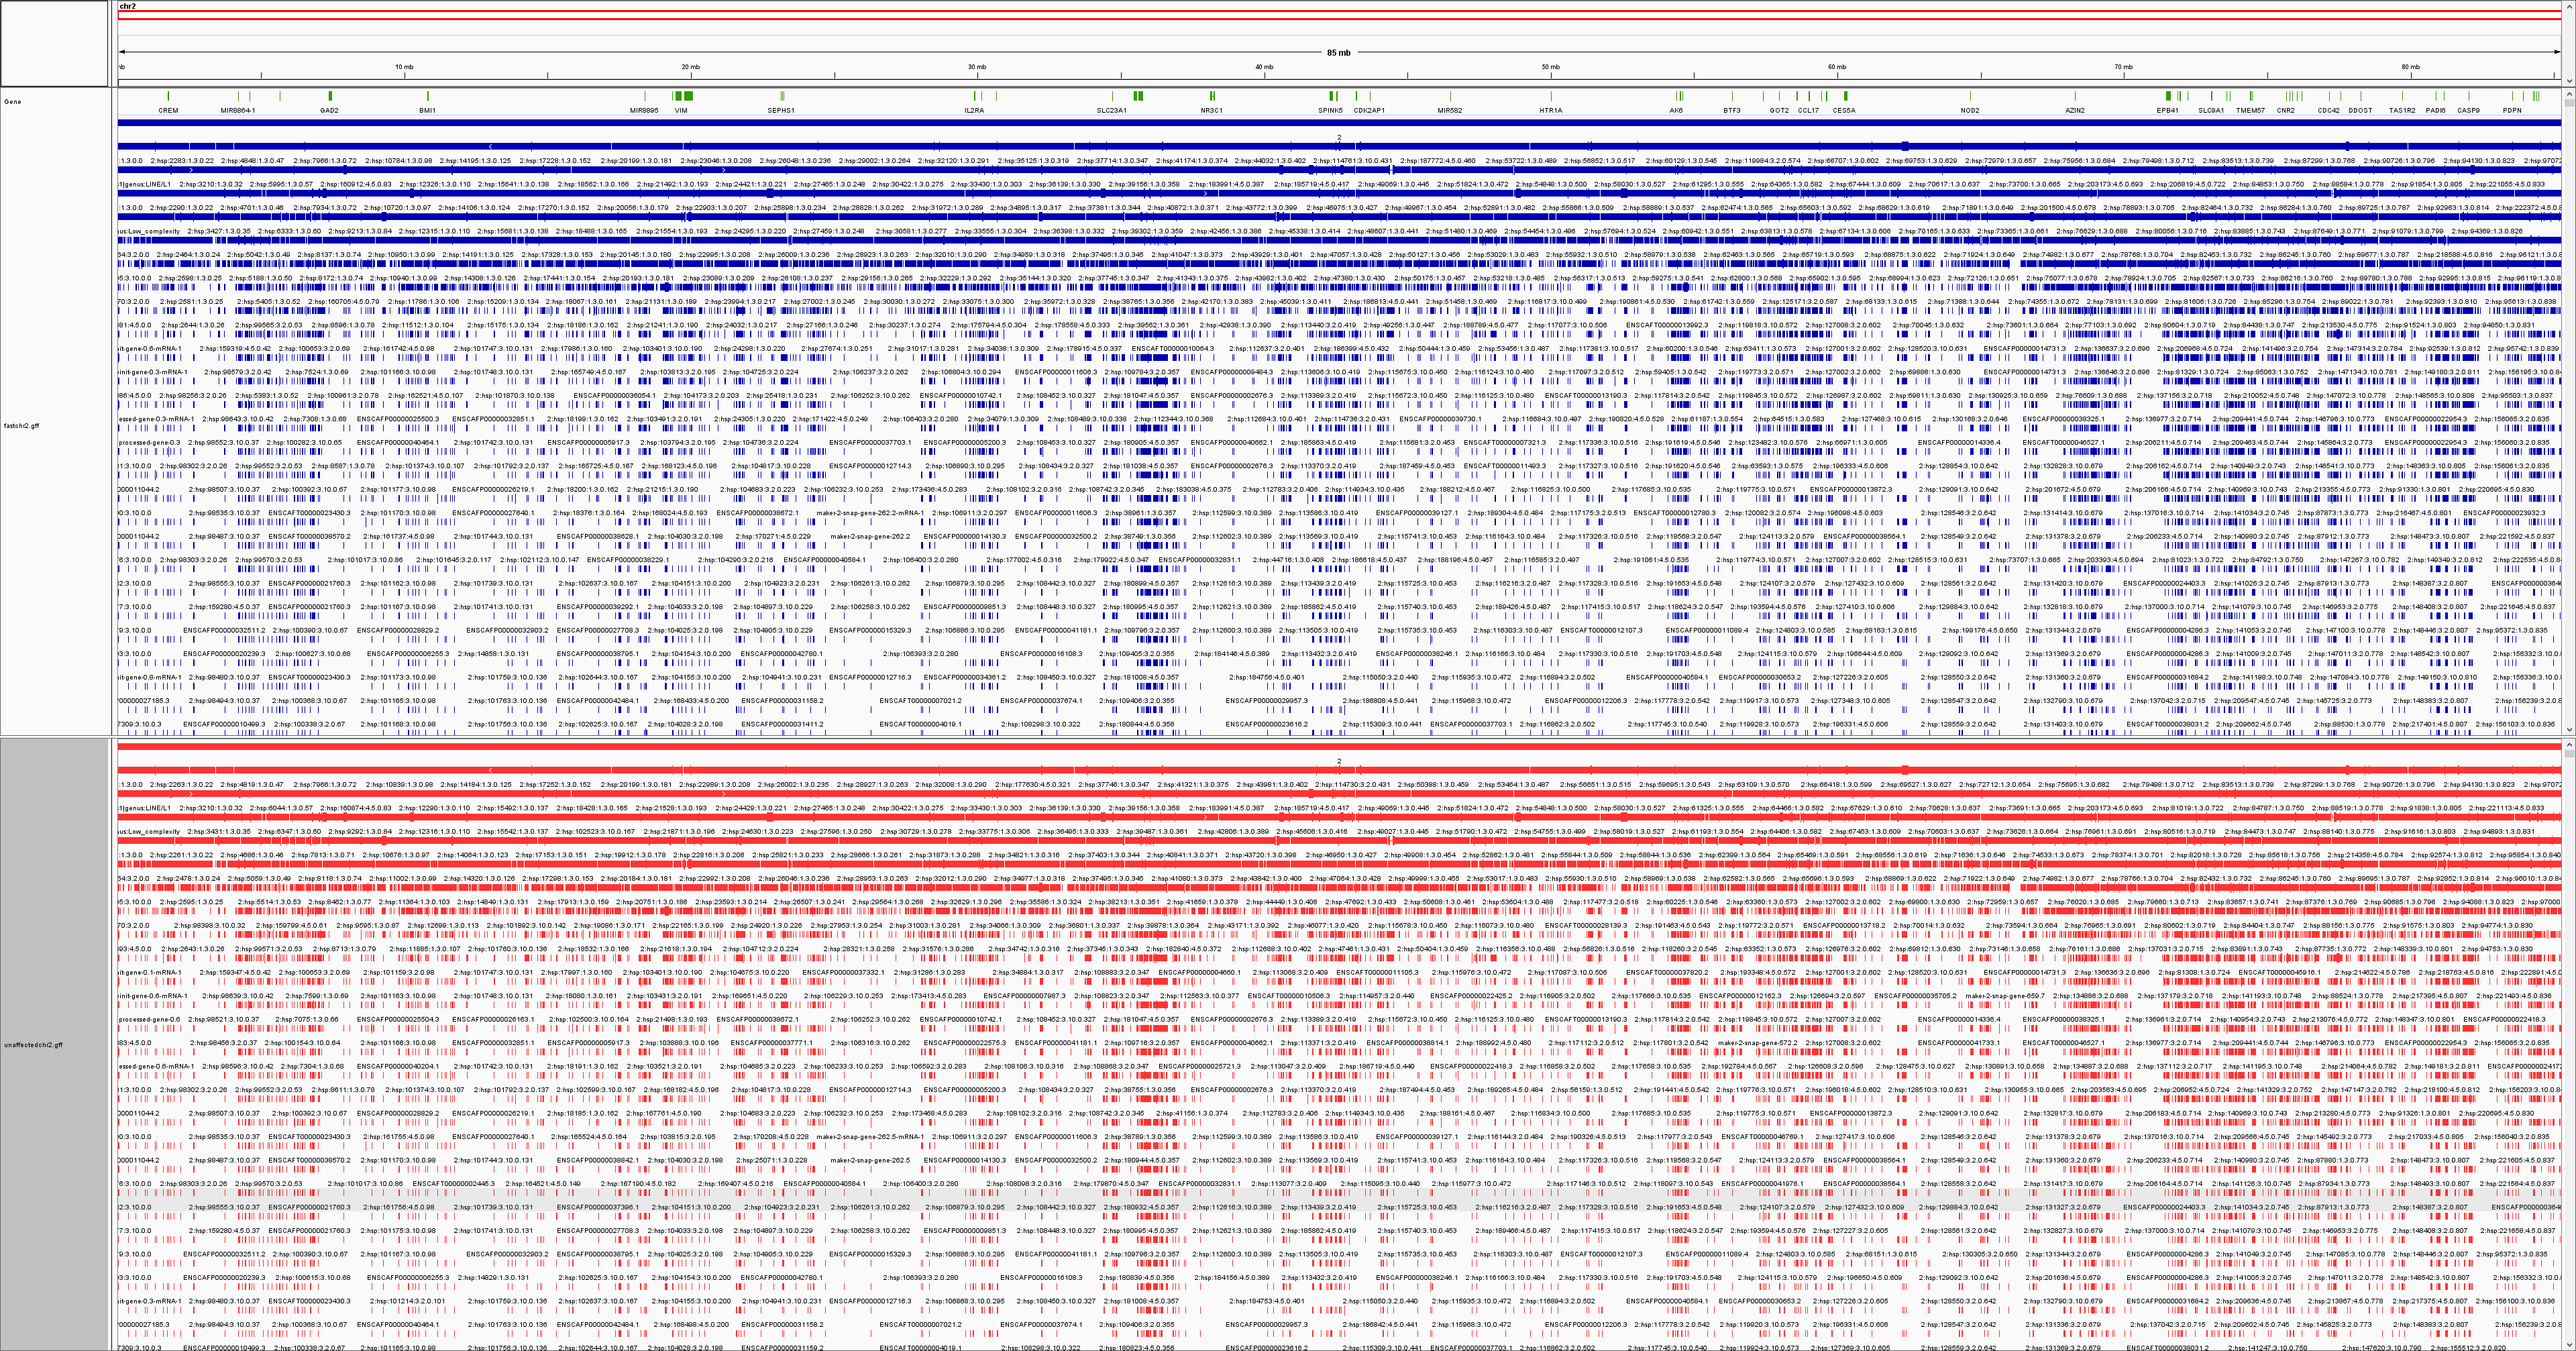
\includegraphics[width=.9\linewidth]{./igv_fast.png}
\caption{\label{fig:igv_fast-vs-unaffected}identical gtfs fast vs unaffected}
\end{figure}

\begin{figure}[htb]
\centering
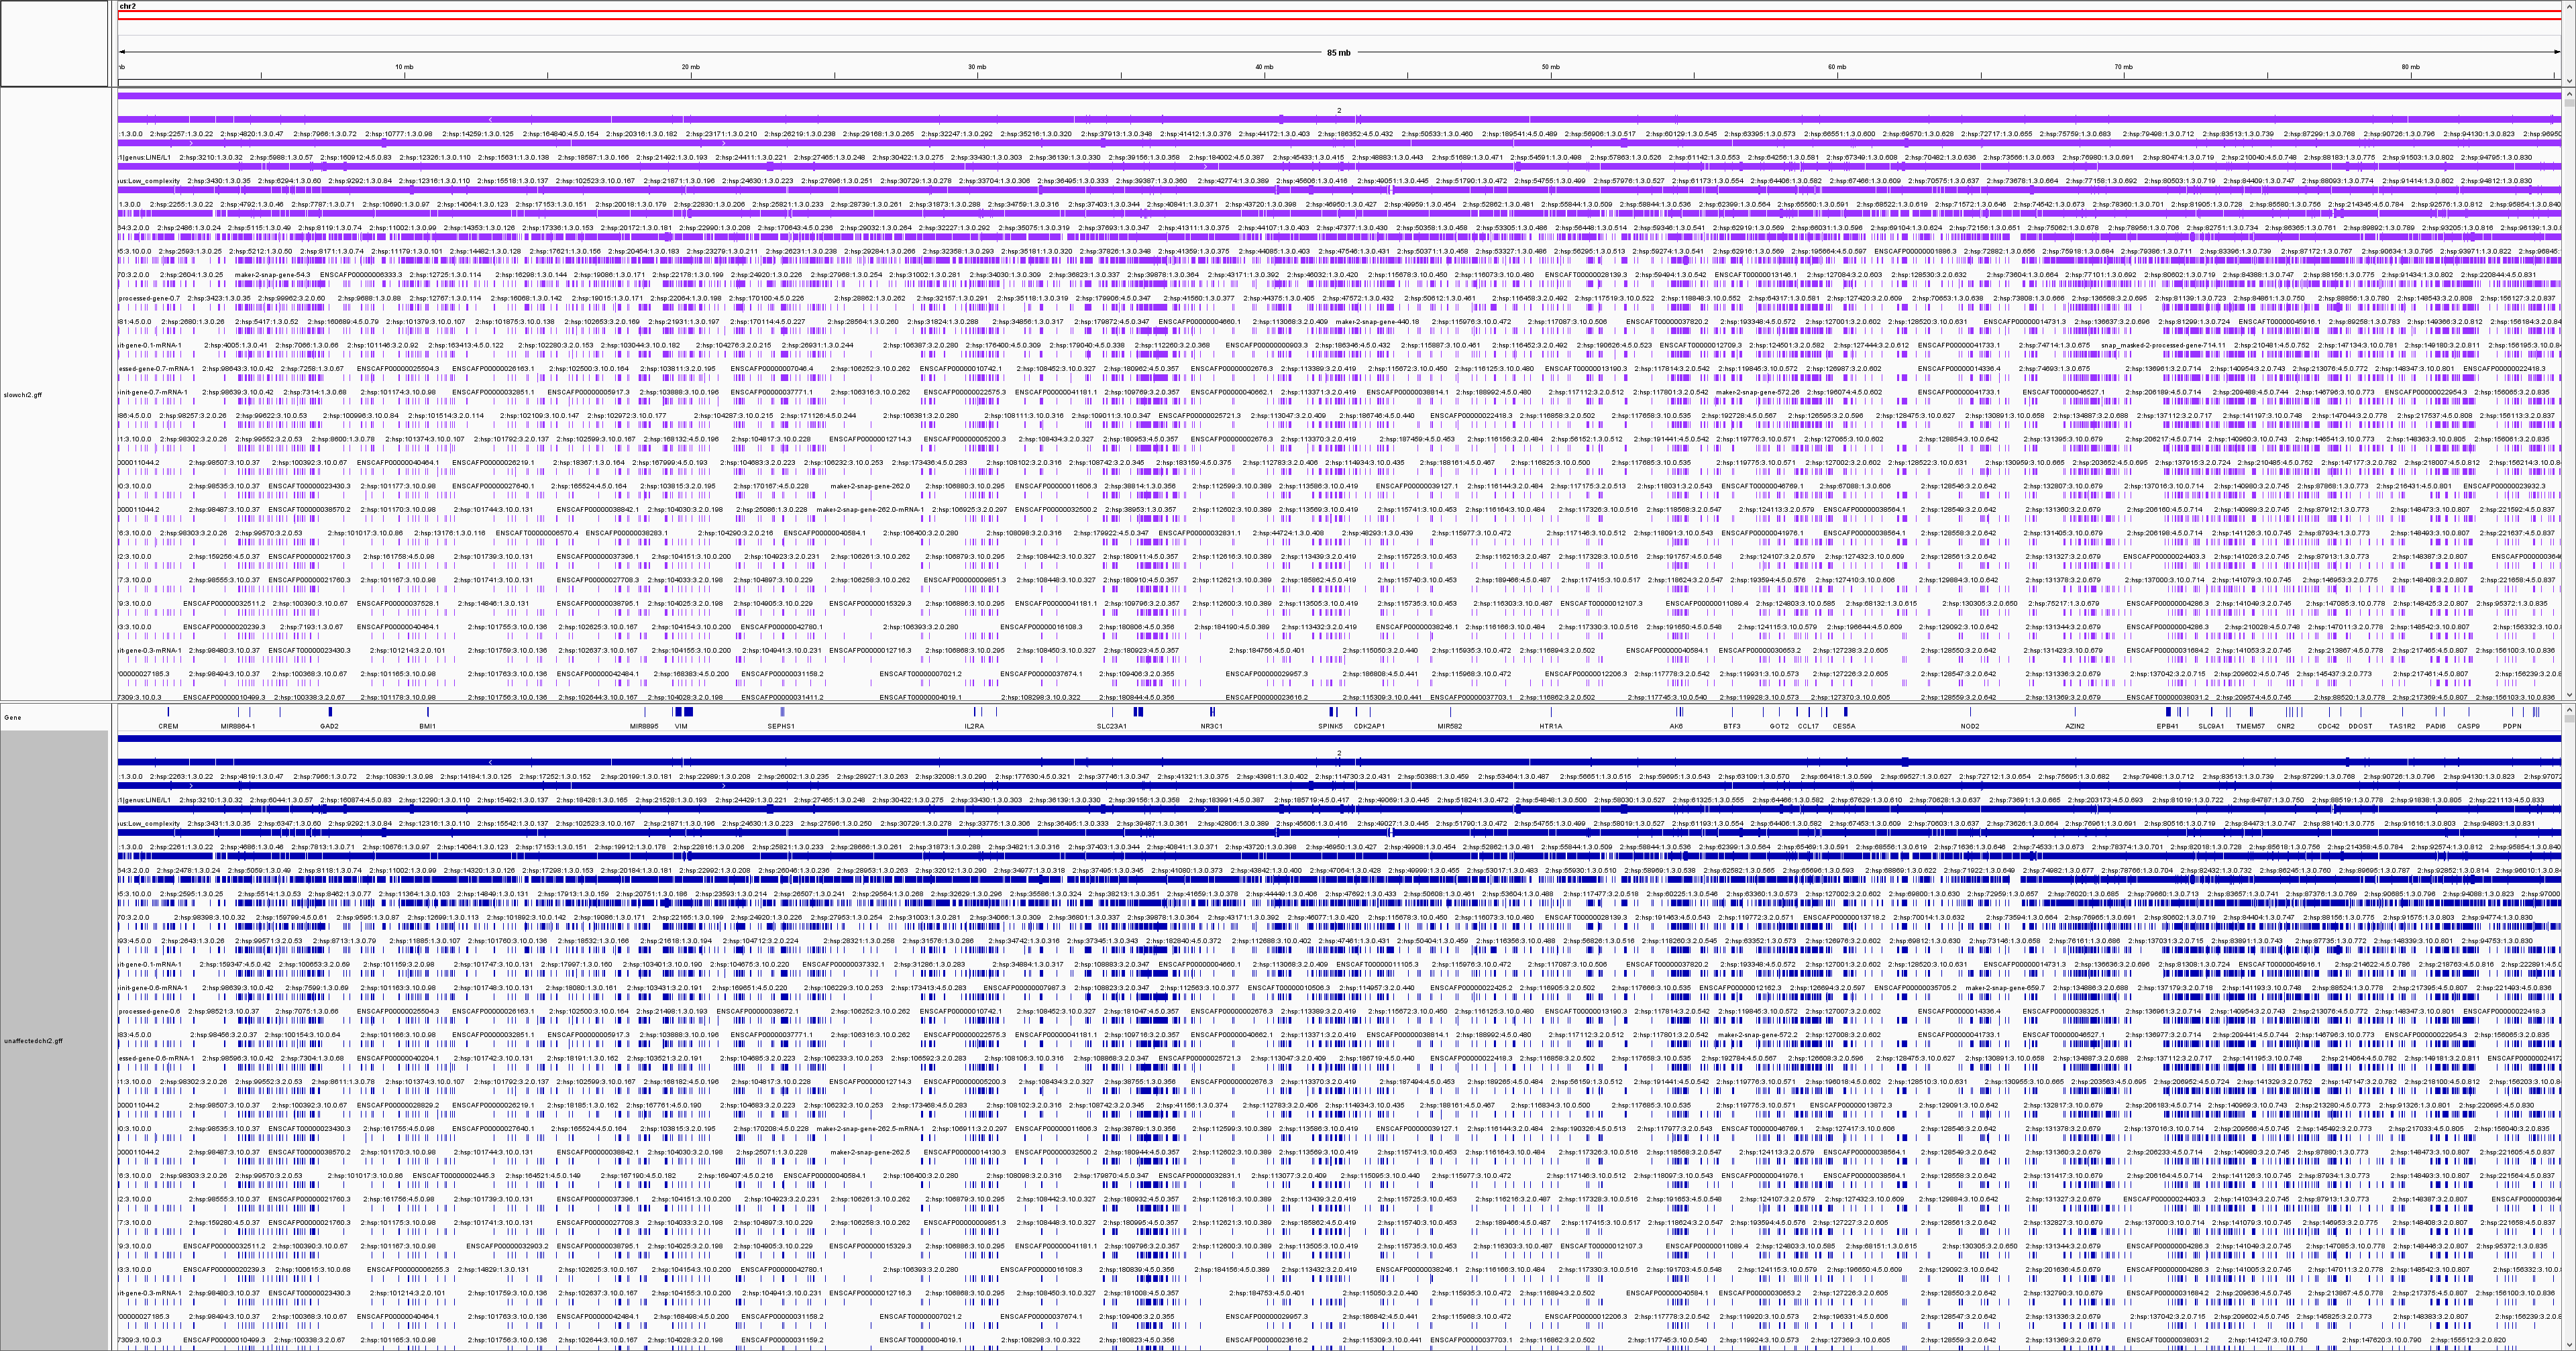
\includegraphics[width=.9\linewidth]{./igv_slow.png}
\caption{\label{fig:igv_slow-vs-unaffected}identical gtfs for slow vs unaffected}
\end{figure}
\href{./table.org}{table.org}
% Emacs 24.5.1 (Org mode 8.2.10)
\end{document}
